\documentclass[xcolor=dvipsnames]{beamer}
\usetheme{presentation}
\usepackage[round]{natbib}
\usepackage{bibentry}
\definecolor{citecolor}{gray}{0.6}
\let\oldcitep\citep
\renewcommand{\citep}[1]{{\color{citecolor}\tiny\oldcitep{#1}}}
\nobibliography*
%\usepackage[cjk]{kotex}
%\usepackage{listings}
\usepackage{tikz}
\usetikzlibrary{arrows.meta}
\tikzset{
    invisible/.style={opacity=0},
    visible on/.style={alt={#1{}{invisible}}},
    alt/.code args={<#1>#2#3}{%
      \alt<#1>{\pgfkeysalso{#2}}{\pgfkeysalso{#3}} % \pgfkeysalso doesn't change the path
    },
}
% ----------------------------- Title & Author ------------------------------ %
\title{Causal Inference with Ordinal Outcomes}
\subtitle{Density Estimation Based Approach}
\author{Chanhyuk Park}
\institute{Washington University in St. Louis}
\date{}

\begin{document}
   \frame{\titlepage}
\begin{frame}{Motivation: The Discretization Problem}
    \begin{itemize}
        \item Experiments to identify causal effects of treatments
        \pause 
        \item Outcomes are usually believed to be continuous in unidimensional space
            \begin{itemize}
                \item Approval ratings \citep{Canes-Wrone2002a, Kriner2009a}
                \item Policy preferences \citep{Scheve2001r, Mayda2005a, Wu2022a}
            \end{itemize}
        \pause
        \item The Problem - How we measure it
    \end{itemize}

    \vspace{0.5cm}

    \centering
    % The Latent Axis Line and its label appear on Step 2 and persist.
    \only<3->{
        \begin{tikzpicture}[font=\sffamily, thick]
            % --- Main Axis (Always Black and No Arrow) ---
            \begin{scope} 
                % Removed '->' to get rid of the arrow
                \draw[very thick, black] (0,0) -- (10,0); 
                \foreach \x in {0, 10} \draw (\x, 0.2) -- (\x, -0.2);
                % Axis Label
                \node[above, yshift=5pt] at (5, 0) {\textbf{The True Outcome}};
            \end{scope}

            % --- Step 3: First Arbitrary Bracketing ---
            \only<4>{
                \begin{scope} 
                    % Partition A Cut-Points
                    \foreach \x in {2, 4.5, 6, 8.5} \draw (\x, 0.2) -- (\x, -0.2);

                    % Brackets (Hanging Arches)
                    \draw (0,-0.2) to [out=-90, in=150] (1, -1.2);
                    \draw (2,-0.2) to [out=-90, in=30] (1, -1.2);
                    
                    \draw (2,-0.2) to [out=-90, in=150] (3.25, -1.2);
                    \draw (4.5,-0.2) to [out=-90, in=30] (3.25, -1.2);

                    \draw (4.5,-0.2) to [out=-90, in=150] (5.25, -1.2);
                    \draw (6,-0.2) to [out=-90, in=30] (5.25, -1.2);
                    
                    \draw (6,-0.2) to [out=-90, in=150] (7.25, -1.2);
                    \draw (8.5,-0.2) to [out=-90, in=30] (7.25, -1.2);
                    
                    \draw (8.5,-0.2) to [out=-90, in=150] (9.25, -1.2);
                    \draw (10,-0.2) to [out=-90, in=30] (9.25, -1.2);

                    % Bottom Labels
                    \node at (1, -1.5) {\scriptsize\itshape Strongly Agree};
                    \node at (3.25, -1.5) {\scriptsize\itshape Agree};
                    \node at (5.25, -1.5) {\scriptsize\itshape Neither};
                    \node at (7.25, -1.5) {\scriptsize\itshape Disagree};
                    \node at (9.25, -1.5) {\scriptsize\itshape Strongly Disagree};
                \end{scope}
            }

            % --- Step 4: Second Arbitrary Bracketing ---
            \only<5>{
                \begin{scope} 
                    % Partition B Cut-Points
                    \foreach \x in {3, 4, 5, 9} \draw (\x, 0.2) -- (\x, -0.2);

                    % Brackets
                    \draw (0,-0.2) to [out=-90, in=150] (1.5, -1.2);
                    \draw (3,-0.2) to [out=-90, in=30] (1.5, -1.2);
                    
                    \draw (3,-0.2) to [out=-90, in=150] (3.5, -1.2);
                    \draw (4,-0.2) to [out=-90, in=30] (3.5, -1.2);

                    \draw (4,-0.2) to [out=-90, in=150] (4.5, -1.2);
                    \draw (5,-0.2) to [out=-90, in=30] (4.5, -1.2);
                    
                    \draw (5,-0.2) to [out=-90, in=150] (7, -1.2);
                    \draw (9,-0.2) to [out=-90, in=30] (7, -1.2);
                    
                    \draw (9,-0.2) to [out=-90, in=150] (9.5, -1.2);
                    \draw (10,-0.2) to [out=-90, in=30] (9.5, -1.2);

                    % Bottom Labels
                    \node at (1.5, -1.5) {\scriptsize\itshape Strongly Agree};
                    \node at (3.5, -1.5) {\scriptsize\itshape Agree};
                    \node at (4.5, -1.5) {\scriptsize\itshape Neither};
                    \node at (7, -1.5) {\scriptsize\itshape Disagree};
                    \node at (9.5, -1.5) {\scriptsize\itshape Strongly Disagree};
                \end{scope}
            }
        \end{tikzpicture}
    }
\end{frame}

\begin{frame}{The Goal}
    \begin{itemize}[<+->]
        \item \textbf{Identification}: \\ 
            Naive causal identification with these "index" may fail \\
            $\implies$ Normalized Latent Treatment Effect (NLTE)
        \item \textbf{Estimation}: \\
            Standard parametric regression is rigid \\
            $\implies$ Flexible, density estimation based estimators
    \end{itemize}
\end{frame}

\begin{frame}{Up To Scale Identification}
    \begin{itemize}[<+->]
        \item We can identify LTE up to scale (Theorem 1)
        \item From the model and data we know:
            $$
            \begin{aligned}
                \mathbb{P}\left(Y(D) \le j\right) &= \mathbb{P}\left(Y^{\ast} \le \alpha_j \right) \\
            \end{aligned}
            $$  
        \item We can construct MLE with using this probability.
        \item However, if we scale $Y^{\ast}$ side by a constant, $c > 0$, we still get the same probability
            $$
            \begin{aligned}
                \mathbb{P}\left(Y(D) \le j\right) &= \mathbb{P}\left(Y^{\ast} \le \alpha_j \right) \\
                &= \mathbb{P}\left(c Y^{\ast} \le c \alpha_j\right) \\
            \end{aligned}
            $$  
    \end{itemize}
\end{frame}

\begin{frame}{Normalization}
    \begin{itemize}[<+->]
        \item Up to scale identification is disappointing
        \item Proper normalization helps interpretation and comparison across models and across samples
        \item Fixing $Var(\varepsilon_{i}) = 1$ is one way
        \item This works as mapping $Y_{i}^{\ast}$ to the space where the variance of the error is a unit / probit space
    \end{itemize}
\end{frame}

\begin{frame}{Common Transformation: Cardinalization and Binarization}
    \begin{itemize}
        \item Cardinalization
            \begin{itemize}
                \item Relies on luck
            \end{itemize}
        \item Binarization
            \begin{itemize}
                \item Lose significant efficiency
                \item Estimate may be sensitive to how you group the ordinal outcomes
            \end{itemize}
    \end{itemize}
\end{frame}

\begin{frame}{Small Example}
    \begin{table}[ht]
        \centering
        \begin{tabular}{c|cc}
            \hline
             & $Y_i^\ast(0)$ & $Y_i^\ast(1)$ \\
            \hline
            A &  1.37 & 0.09 \\
            B & -0.56 & 1.71 \\
            C &  0.36 & 0.11 \\
            D &  0.63 & 2.22 \\
            E &  0.40 & 0.14 \\
            \hline
        \end{tabular}
        \label{tab:latent_example}
    \end{table}
    \begin{itemize}
        \item The LTE in the latent preference space is: $0.41$
    \end{itemize}
\end{frame}

\begin{frame}{Small Example -- Cardinalization}
    \begin{itemize}
        \item Suppose two transformation functions: $g_{a}$ and $g_{b}$
        \item Both are monotone, but with different thresholds ($\alpha_{j}$)
    \end{itemize}
    \begin{table}[ht]
        \centering
        \begin{tabular}{c|cc|cc}
            \hline
            & \multicolumn{2}{c|}{$g_a$} & \multicolumn{2}{c}{$g_b$} \\
            & $Y_{i,g_a}(0)$ & $Y_{i,g_a}(1)$ & $Y_{i,g_b}(0)$ & $Y_{i,g_b}(1)$ \\
            \hline
            A & Agree          & Agree          & Agree          & Disagree \\
            B & Neither        & Agree          & Disagree       & Agree    \\
            C & Agree          & Agree          & Neither        & Disagree \\
            D & Agree          & Strongly Agree & Neither        & Agree    \\
            E & Agree          & Agree          & Neither        & Disagree \\
            \hline
        \end{tabular}
        \label{tab:g_example}
    \end{table}
\end{frame}

\begin{frame}{Small Example -- Cardinalization}
    \begin{itemize}
        \item A researcher impose common cardinalization of 1 to 5,
        \item In case the true transformation is $g_{a}$, the estimate is $-0.4$
        \item In case the true transformation is $g_{b}$, the estimate is $0.2$
        \item Without compelling reason to impose such numeric labels, cardinalization relies on pure luck
    \end{itemize}
\end{frame}

\begin{frame}{Estimation}
    \begin{itemize}
        \item There has been tools for ordinal outcomes
        \item Standard parametric approaches such as Ordered Probit and Ordered Logit
        \item Two estimators based on density estimation techniques
    \end{itemize}
\end{frame}

\begin{frame}{Ordered Logit and Probit}
    \begin{itemize}
        \item Assume that the error term follows a specific distribution (Logistic and Standard Normal)
        \item And use maximum likelihood to estimate the coefficients
        \item Identify coefficients up to scale
        \item Once distributional assumption is violated, inconsistent
    \end{itemize}
\end{frame}

\begin{frame}{Ordered Logit and Probit}
\begin{itemize}
    \item The true log-likelihood is:

    \[
    \begin{aligned}
    \ell(\alpha,\beta,\tau)
    =\;
    &\sum_{i=1}^n \sum_{j=0}^J  
        1_{\{Y_i = j\}}
        \Bigg\{
            \log F\!\left(
                \alpha_j 
                - f(X_i,\beta)
                + D_i^\top \tau
            \right)
    \\
    &\qquad\qquad\qquad
            -\;
            \log F\!\left(
                \alpha_{j-1}
                - f(X_i,\beta)
                + D_i^\top \tau
            \right)
        \Bigg\}
    \end{aligned}
    \]

    \item $F$ is the CDF of the true error.
    \item If $F$ is not standard normal or standard logistic, MLE is inconsistent.
    \item The error is never known, and omitted or unobserved confounder may also distort the error
\end{itemize}
\end{frame}

\begin{frame}{Alternative: Estimate the $F$}
    \begin{itemize}
        \item Instead of assuming a specific $F$, we can estimate as $\hat{F}$
        \item Then the log-likelihood becomes:
            \[
            \begin{aligned}
                \hat{\ell}(\alpha,\beta,\tau)
            =\;
            &\sum_{i=1}^n \sum_{j=0}^J  
                1_{\{Y_i = j\}}
                \Bigg\{
                    \log \hat{F}\!\left(
                        \alpha_j 
                        - f(X_i,\beta)
                        + D_i^\top \tau
                    \right)
            \\
            &\qquad\qquad\qquad
                    -\;
                    \log \hat{F}\!\left(
                        \alpha_{j-1}
                        - f(X_i,\beta)
                        + D_i^\top \tau
                    \right)
                \Bigg\}
            \end{aligned}
            \]
        \item I propose to use two density estimation methods: KDE and Normalizing Flows
    \end{itemize}
\end{frame}

\begin{frame}{Kernel Density Estimation}
    \begin{itemize}
        \item Nonparametric method
        \item Smooth each observation using a kernel (usually Gaussian)
            $$
                \hat f(x)
= \frac{1}{n h} \sum_{i=1}^n K\!\left( \frac{x - X_i}{h} \right)
            $$ 
        \item Generally, the moderate bandwidth ensures enough convergence rate for $\sqrt{n}$ consistency for the main estimator (semiparametric efficiency)
    \end{itemize}
\end{frame}

\begin{frame}{Normalizing Flows}
    \begin{itemize}
        \item A flexible class of models that transform complex continuous density to simple base density (usually Gaussian)
        \item Use the change-of-variable formula
            $$
                f_\theta(h)
                = f_Z\bigl(T_\theta^{-1}(h)\bigr)
                \left|\det \diff T_\theta^{-1}(h)\right|,
            $$
        \item $T_{\theta}$ is a set of \textit{invertible} transformation
        \item Rational Quadratic Spline Flow
        \item Since this is fully parametric, for finite $\theta$, MLE ensures $\sqrt{n}$ consistency
    \end{itemize}
\end{frame}

\begin{frame}{Simulation}
    \begin{itemize}
        \item Ordered Probit Ordered Logit and NF based only
        \item Errors: Standard Normal and Log Normal distribution
        \item A binary treatment randomized 
        \item Covariates: One binary and three continuous (following normal distribution)
        \item Thresholds: $-2, -1, 1, 2.5$ $\rightarrow$ 5 categories
        \item Sample sizes: 200, 500, 1000, 2000
        \item 200 Replications
    \end{itemize}
\end{frame}

\begin{frame}{Simulation}
\begin{figure}
    \begin{tabular}{cc}
        \includegraphics[width=0.45\textwidth]{../figures/latent_space_normal_N1000000.png} & \includegraphics[width=0.45\textwidth]{../figures/latent_space_lognormal_N1000000.png}\\
    \end{tabular}
\end{figure}
\end{frame}

\begin{frame}{Simulation -- Normal Case}
    \begin{itemize}
        \item True treatment size: 1.0
    \end{itemize}
\begin{figure}
    \begin{tabular}{cc}
        \includegraphics[width=0.45\textwidth]{../figures/expect_bias_oprobit_ologit_flow_normal_OLS.pdf} & \includegraphics[width=0.45\textwidth]{../figures/expect_rmse_oprobit_ologit_flow_normal_OLS.pdf}\\
    \end{tabular}
\end{figure}
\end{frame}

\begin{frame}{Simulation -- Lognormal Case}
    \begin{itemize}
        \item True treatment size: 0.46
    \end{itemize}
\begin{figure}
    \begin{tabular}{cc}
        \includegraphics[width=0.45\textwidth]{../figures/expect_bias_oprobit_ologit_flow_lognormal_OLS.pdf} & \includegraphics[width=0.45\textwidth]{../figures/expect_rmse_oprobit_ologit_flow_lognormal_OLS.pdf}\\
    \end{tabular}
\end{figure}
\end{frame}

\begin{frame}{Conclusion}
    \begin{itemize}
        \item With ordinal outcomes, treatment effects can only be identified up to scale
        \item Cardinalization and Binarization have its pitfalls
        \item Standard parametric approaches relies on strong distributional assumption
        \item KDE and NF based approaches may provide flexible ways to estimate the true effects
        \item For KDE, the normalization of coefficients is an issue...
        \item For NF, Hyperparameter selection is an issue, trying to automatically adjust it while traing
    \end{itemize}
\end{frame}

\bibliographystyle{plainnat}
\nobibliography{/Users/chanhyuk/Documents/MyLibrary}

\end{document}
